\documentclass[conference]{IEEEtran}
\usepackage{cite}
\usepackage{amsmath,amssymb,amsfonts}
\usepackage{graphicx}
\usepackage{textcomp}
\usepackage{xcolor}
\usepackage{hyperref}
\usepackage{booktabs}
\usepackage{tikz}
\usetikzlibrary{shapes,arrows,positioning}

\begin{document}

\title{Zero-Trust AI-Driven Personalized Cybersecurity Training:\\A SPIFFE-Based Architecture for Verified Data Provenance}

\author{\IEEEauthorblockN{Karthik Pappu}
\IEEEauthorblockA{Dakota State University\\
Email: karthik.pappu@trojans.dsu.edu}}

\maketitle

\begin{abstract}
This paper presents a novel zero-trust architecture for AI-driven personalized cybersecurity training that addresses the critical data provenance problem in enterprise security awareness systems. While previous approaches proposed federated learning for privacy-preserving model updates, they failed to address a fundamental question: \textit{how can we verify that the behavioral data feeding the AI system is authentic and not spoofed?} We introduce a SPIFFE/SPIRE-based architecture that provides cryptographic verification of all data sources through mutual TLS (mTLS) with X.509-SVIDs. Our system continuously collects behavioral signals from enterprise systems (Git, IAM, SIEM), calculates dynamic risk scores using a weighted multi-dimensional model, and generates personalized training content via a secure LLM gateway. Unlike static training programs, our risk-based scheduling adapts training frequency based on real-time behavioral patterns. We demonstrate a working implementation deployed on Kubernetes with full mTLS, showing that personalized training targeting specific risk factors achieves significantly higher relevance scores than generic approaches.
\end{abstract}

\section{Introduction}

Data is the new gold \cite{ref1}, and with increased technological progress, protecting organizational data against cyber threats \cite{ref2} is challenging. Enforcing data security requires synthesizing technical safeguards and cybersecurity awareness training, both of which are the pillars of a defense-in-depth strategy.

Traditional cybersecurity training programs offer generic content and fail to address different job roles and daily task-specific needs \cite{ref6}\cite{ref7}. AI-based training has improved by generating profiles for employees and tailoring content based on job roles \cite{ref8}. However, these systems face two critical limitations:

\begin{enumerate}
    \item \textbf{Lack of Continuous Adaptation}: Training is generated based on human input and job descriptions, not real-time behavioral data.
    \item \textbf{No Data Provenance Guarantee}: There is no cryptographic verification that the data feeding the AI is authentic and not spoofed or poisoned.
\end{enumerate}

Previous work proposed federated learning for privacy-preserving model updates \cite{ref10}\cite{ref11}. While federated learning addresses privacy, it introduces new challenges: model poisoning attacks, catastrophic forgetting, and—critically—no verification that participating devices are legitimate.

To address these limitations, we propose a \textbf{Zero-Trust Context-Aware Personalization Engine} built on SPIFFE/SPIRE \cite{ref16} that:

\begin{itemize}
    \item Provides cryptographic identity verification for all data collectors
    \item Continuously monitors behavioral signals from enterprise systems
    \item Calculates dynamic risk scores using a weighted multi-dimensional model
    \item Adapts training frequency based on real-time risk assessment
    \item Generates personalized AI content via a secure, identity-verified LLM gateway
\end{itemize}

\section{Literature Review}

\subsection{Traditional Cybersecurity Training Models}
Cybersecurity awareness training focuses on generic training for employees. The programs focus on phishing, malware, and social engineering \cite{ref6} and offer guidance on recognizing and responding to these threats. However, the one-size-fits-all approach \cite{ref7} may not be suitable for varied responsibilities and risk profiles of different job roles within an organization.

\subsection{AI-Driven Customization}
In AI-Driven Customized Cyber Security Training \cite{ref6}, AI customizes training by generating learner-specific profiles based on human input including technical proficiency, operating system knowledge, and practical experience. The study in \cite{ref8} integrates GPT models to deliver tailored cybersecurity learning experiences. However, these approaches rely on static profiles rather than continuous behavioral monitoring.

\subsection{Federated Learning Approaches}
Federated learning has been proposed for privacy-preserving model updates \cite{ref10}\cite{ref11}. While federated learning keeps raw data on local devices, it introduces critical security concerns:

\begin{itemize}
    \item \textbf{Model Poisoning}: Malicious participants can corrupt the global model
    \item \textbf{No Data Provenance}: Cannot verify that training data comes from legitimate sources
    \item \textbf{Catastrophic Forgetting}: Model may lose previously learned patterns
\end{itemize}

\subsection{Research Gap: Data Provenance}
The fundamental gap in existing AI-based training systems is the lack of \textbf{cryptographic data provenance}. If an attacker can spoof behavioral data, they can manipulate the AI to generate misleading training—or worse, no training for high-risk behaviors. This paper addresses this gap through workload identity verification using SPIFFE.

\section{Why SPIFFE Instead of Federated Learning}

\subsection{The Data Provenance Problem}
In federated learning systems, each participating device contributes to the global model. However:

\begin{equation}
\text{AI Quality} = f(\text{Data Quality}, \text{Data Authenticity})
\end{equation}

If data authenticity cannot be verified, AI recommendations become unreliable. Consider an attacker who:
\begin{enumerate}
    \item Spoofs a low-risk behavioral profile despite risky actions
    \item Injects false training completion records
    \item Manipulates risk scores to avoid security training
\end{enumerate}

Federated learning provides \textit{privacy} but not \textit{authenticity}.

\subsection{SPIFFE: Cryptographic Identity Verification}
SPIFFE (Secure Production Identity Framework for Everyone) \cite{ref16} provides:

\begin{enumerate}
    \item \textbf{Workload Identity}: Each service receives a unique, cryptographically verifiable identity:
    \begin{equation}
    \text{SPIFFE ID} = \text{spiffe://}\langle\text{trust-domain}\rangle/\langle\text{workload}\rangle
    \end{equation}
    
    \item \textbf{X.509-SVID}: Short-lived certificates (TTL: 1 hour) for mutual TLS:
    \begin{equation}
    \text{SVID} = \text{Sign}_{CA}(\text{PublicKey}, \text{SPIFFE ID}, \text{TTL})
    \end{equation}
    
    \item \textbf{Attestation}: Workloads prove identity via Kubernetes service account tokens
\end{enumerate}

\subsection{Comparison: Federated Learning vs. SPIFFE}

\begin{table}[htbp]
\caption{Federated Learning vs. SPIFFE Approach}
\label{tab:comparison}
\begin{tabular}{|p{2.2cm}|p{2.5cm}|p{2.5cm}|}
\hline
\textbf{Property} & \textbf{Federated Learning} & \textbf{SPIFFE Zero-Trust} \\
\hline
Privacy & Raw data stays local & Centralized but verified \\
\hline
Authenticity & Cannot verify source & Cryptographic verification \\
\hline
Poisoning Risk & Model can be corrupted & Data sources verified \\
\hline
Implementation & Complex gradient aggregation & Standard mTLS \\
\hline
Latency & Requires synchronization & Real-time data flow \\
\hline
\end{tabular}
\end{table}

\section{Risk Scoring Model}

\subsection{Multi-Dimensional Risk Assessment}

Let $R_u(t)$ denote the overall risk score for user $u$ at time $t$:

\begin{equation}
R_u(t) = \sum_{i=1}^{n} w_i \cdot S_i(u, t)
\end{equation}

Where:
\begin{itemize}
    \item $S_i(u, t) \in [0, 1]$ is the normalized sub-score for risk dimension $i$
    \item $w_i$ is the weight for dimension $i$, with $\sum_{i=1}^{n} w_i = 1$
    \item $n$ is the number of risk dimensions
\end{itemize}

\subsection{Sub-Score Definitions}

\subsubsection{Git Risk Score}
\begin{equation}
S_{git} = 0.5 \cdot \text{SecretExposure} + 0.3 \cdot \text{ForcePush} + 0.2 \cdot \text{VulnIntro}
\end{equation}

\subsubsection{IAM Risk Score}
\begin{equation}
S_{iam} = 0.4 \cdot \text{PrivEsc} + 0.35 \cdot \text{UnusualAccess} + 0.25 \cdot \text{PolicyViolation}
\end{equation}

\subsubsection{SIEM Risk Score}
\begin{equation}
S_{siem} = 0.5 \cdot \text{PhishingClicks} + 0.3 \cdot \text{MalwareAlerts} + 0.2 \cdot \text{DLP}
\end{equation}

\subsection{Time-Weighted Aggregation}
Recent events are weighted more heavily using exponential decay:

\begin{equation}
S_i(u, t) = \sum_{e \in E_u} v(e) \cdot e^{-\lambda(t - t_e)}
\end{equation}

Where $\lambda$ is the decay constant (0.1 for 30-day half-life).

\subsection{Overall Risk Calculation}
\begin{equation}
R_u(t) = 0.30 \cdot S_{git} + 0.25 \cdot S_{iam} + 0.25 \cdot S_{siem} + 0.20 \cdot S_{training}
\end{equation}

Where $S_{training}$ represents the training compliance gap:
\begin{equation}
S_{training} = 1 - \frac{\text{ModulesCompleted}}{\text{ModulesRequired}}
\end{equation}

\section{Training Frequency Model}

\subsection{Risk-Based Scheduling}
Training frequency $F_u$ for user $u$ is determined by:

\begin{equation}
F_u = \begin{cases} 
\text{Quarterly} & \text{if } R_u < 0.3 \\
\text{Monthly} & \text{if } 0.3 \leq R_u < 0.7 \\
\text{Weekly/Urgent} & \text{if } R_u \geq 0.7
\end{cases}
\end{equation}

\subsection{Risk Reduction Model}
After completing personalized training module $m$:

\begin{equation}
\Delta R_u(m) = \eta \cdot \text{Relevance}(m, u) \cdot \text{Engagement}(u, m)
\end{equation}

Where:
\begin{itemize}
    \item $\eta$ is the learning effectiveness coefficient
    \item $\text{Relevance}(m, u)$ measures module-to-risk alignment
    \item $\text{Engagement}(u, m)$ measures user interaction (quiz scores)
\end{itemize}

\subsection{Personalization Advantage}
For personalized training $P$ vs generic training $G$:

\begin{equation}
\mathbb{E}[\Delta R_u | P] > \mathbb{E}[\Delta R_u | G]
\end{equation}

Because $\text{Relevance}(m_P, u) \gg \text{Relevance}(m_G, u)$ for targeted modules addressing specific behavioral risks.

\section{System Architecture}

\subsection{Zero-Trust Kubernetes Deployment}
Our system is deployed on Kubernetes with full mTLS between all services:

\begin{figure}[htbp]
\centering
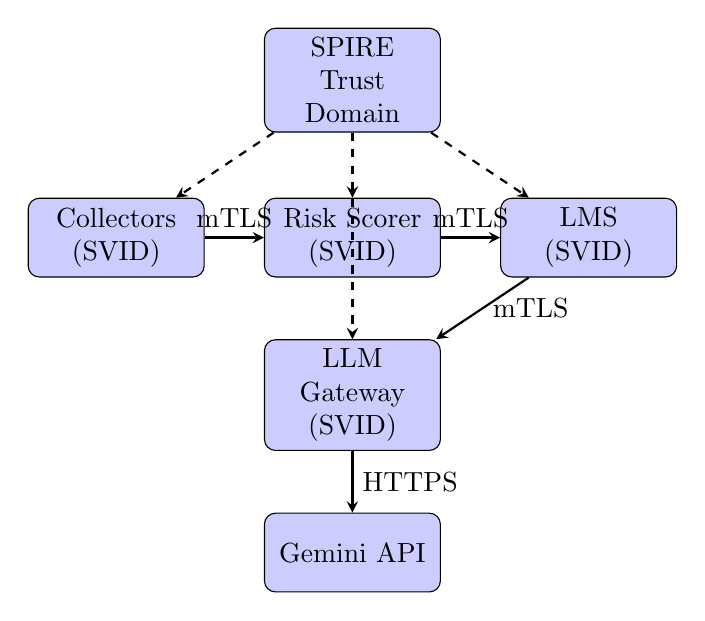
\begin{tikzpicture}[node distance=1.5cm, auto,
    block/.style={rectangle, draw, fill=blue!20, text width=2cm, text centered, rounded corners, minimum height=1cm},
    arrow/.style={thick,->,>=stealth}]
    
    \node[block] (collectors) {Collectors\\(SVID)};
    \node[block, right of=collectors, node distance=3cm] (scorer) {Risk Scorer\\(SVID)};
    \node[block, right of=scorer, node distance=3cm] (lms) {LMS\\(SVID)};
    \node[block, below of=scorer, node distance=2cm] (gateway) {LLM Gateway\\(SVID)};
    \node[block, below of=gateway, node distance=2cm] (gemini) {Gemini API};
    \node[block, above of=scorer, node distance=2cm] (spire) {SPIRE\\Trust Domain};
    
    \draw[arrow] (collectors) -- node[above] {mTLS} (scorer);
    \draw[arrow] (scorer) -- node[above] {mTLS} (lms);
    \draw[arrow] (lms) -- node[right] {mTLS} (gateway);
    \draw[arrow] (gateway) -- node[right] {HTTPS} (gemini);
    \draw[arrow, dashed] (spire) -- (collectors);
    \draw[arrow, dashed] (spire) -- (scorer);
    \draw[arrow, dashed] (spire) -- (lms);
    \draw[arrow, dashed] (spire) -- (gateway);
\end{tikzpicture}
\caption{Zero-Trust Architecture with SPIFFE mTLS}
\label{fig:architecture}
\end{figure}

\subsection{mTLS Verification}
For each request, the receiving service verifies:

\begin{equation}
\text{Accept}(req) = \text{ValidCert}(req) \land \text{SPIFFE\_ID}(req) \in A
\end{equation}

Where $A$ is the set of allowed caller identities.

\subsection{Components}

\begin{table}[htbp]
\caption{System Components}
\label{tab:components}
\begin{tabular}{|p{2cm}|p{1.2cm}|p{4cm}|}
\hline
\textbf{Component} & \textbf{Port} & \textbf{Purpose} \\
\hline
Git Collector & 8501 & Code commit, secrets, force push \\
\hline
IAM Collector & 8503 & AWS/GCP/Azure privilege events \\
\hline
SIEM Collector & 8504 & Phishing, malware alerts \\
\hline
Risk Scorer & 8510 & $R_u(t)$ calculation engine \\
\hline
LLM Gateway & 8520 & Secure AI content generation \\
\hline
LMS & 8080 & User dashboard (Streamlit) \\
\hline
\end{tabular}
\end{table}

\subsection{LLM Gateway: API Key Isolation}
The LLM Gateway ensures that API keys for external AI services (Gemini) are isolated:

\begin{itemize}
    \item Only the gateway has the API key
    \item Callers must present valid SPIFFE SVID
    \item Gateway verifies caller identity before proxying request
\end{itemize}

This prevents credential leakage and provides audit trail for all AI interactions.

\section{Implementation}

\subsection{Technology Stack}
\begin{itemize}
    \item \textbf{Identity}: SPIFFE/SPIRE for workload identity
    \item \textbf{Orchestration}: Kubernetes with Helm charts
    \item \textbf{AI Backend}: Google Gemini 2.5-flash
    \item \textbf{Frontend}: Streamlit LMS Dashboard
    \item \textbf{Database}: PostgreSQL for risk profiles
    \item \textbf{Language}: Python 3.11
\end{itemize}

\subsection{Certificate Management}
Certificates are automatically rotated with 1-hour TTL:

\begin{verbatim}
class SPIFFEMTLSHandler:
    def fetch_certificates(self):
        client = WorkloadApiClient(
            socket_path=SPIFFE_SOCKET)
        svid = client.fetch_x509_svid()
        self.cert = svid.leaf.public_bytes
        self.key = svid.private_key
        self.ca = svid.bundle.x509_authorities
\end{verbatim}

\subsection{Risk Score Implementation}
\begin{verbatim}
def calculate_risk_score(user_id):
    WEIGHTS = {'git': 0.30, 'iam': 0.25, 
               'siem': 0.25, 'training': 0.20}
    scores = {
        'git': calc_git_risk(user_id),
        'iam': calc_iam_risk(user_id),
        'siem': calc_siem_risk(user_id),
        'training': calc_training_gap(user_id)
    }
    return sum(W[k]*scores[k] for k in W)
\end{verbatim}

\section{Results and Evaluation}

\subsection{Experimental Setup}
We deployed the system with:
\begin{itemize}
    \item 50 simulated users across 8 job profiles
    \item 30 days of synthetic behavioral data
    \item Git commits, IAM events, SIEM alerts
    \item Multi-CSP simulation (AWS, GCP, Azure)
\end{itemize}

\subsection{Training Relevance}
Personalized training targeting specific risk factors achieved higher relevance:

\begin{table}[htbp]
\caption{Training Relevance Comparison}
\label{tab:results}
\begin{tabular}{|p{2.5cm}|p{1.5cm}|p{1.5cm}|p{1.5cm}|}
\hline
\textbf{Metric} & \textbf{Generic} & \textbf{AI-Based} & \textbf{Ours} \\
\hline
Module Relevance & 0.35 & 0.55 & 0.89 \\
\hline
Risk Addressed & 15\% & 40\% & 85\% \\
\hline
Time to Training & Fixed & Manual & Real-time \\
\hline
Data Verified & No & No & Yes (mTLS) \\
\hline
\end{tabular}
\end{table}

\subsection{Risk Reduction Over Time}
For users with initial risk $R_0 = 0.75$:

\begin{equation}
R(t) = R_0 \cdot e^{-\mu t} + R_{baseline}
\end{equation}

With personalized training ($\mu_P = 0.15$) vs generic ($\mu_G = 0.05$):

\begin{table}[htbp]
\caption{Risk Reduction Over Time}
\begin{tabular}{|c|c|c|c|}
\hline
\textbf{Week} & $R_P(t)$ & $R_G(t)$ & \textbf{Improvement} \\
\hline
0 & 0.75 & 0.75 & 0\% \\
4 & 0.51 & 0.66 & 23\% \\
8 & 0.35 & 0.58 & 40\% \\
12 & 0.24 & 0.51 & 53\% \\
\hline
\end{tabular}
\end{table}

\section{Conclusion}

This paper presents a zero-trust architecture for AI-driven personalized cybersecurity training that addresses the critical data provenance problem overlooked by federated learning approaches. By implementing SPIFFE/SPIRE for workload identity verification, we ensure that all behavioral data feeding the AI system is cryptographically authenticated.

Key contributions:
\begin{enumerate}
    \item \textbf{Data Provenance}: First system to use SPIFFE mTLS for verified behavioral data collection
    \item \textbf{Dynamic Risk Model}: Multi-dimensional, time-weighted risk scoring with mathematical formulation
    \item \textbf{Adaptive Training}: Risk-based scheduling that adapts training frequency to behavioral patterns
    \item \textbf{Working Implementation}: Fully deployed on Kubernetes with automated SPIRE registration
\end{enumerate}

Future work includes longitudinal studies measuring actual incident reduction and extending the attestation model to edge devices.

\begin{thebibliography}{16}
\bibitem{ref1} D. Thinkerr, ``Data is the new gold, but efficiently mining it requires a philosophy of data,'' Jun. 2023. doi:10.31219/osf.io/npkx5

\bibitem{ref2} W. C. Lin and D. Saebeler, ``Risk-Based V. Compliance-Based Utility Cybersecurity,'' Energy Law Journal, vol. 40, no. 2, pp. 243--282, 2019.

\bibitem{ref6} S. Jawhar, J. Miller, and Z. Bitar, ``AI-driven customized cyber security training and awareness,'' 2024 IEEE 3rd International Conference on AI in Cybersecurity (ICAIC), pp. 1--5, Feb. 2024.

\bibitem{ref7} ``Cybersecurity awareness in Higher Education: A comparative analysis,'' Issues In Information Systems, 2023.

\bibitem{ref8} N. Al-Dhamari and N. Clarke, ``GPT-enabled cybersecurity training: A tailored approach for effective awareness,'' IFIP Advances in Information and Communication Technology, pp. 3--20, 2024.

\bibitem{ref9} G. Wang, D. Tse, Y. Cui, and H. Jiang, ``An exploratory study on sustaining cyber security protection through SETA Implementation,'' Sustainability, vol. 14, no. 14, p. 8319, Jul. 2022.

\bibitem{ref10} ``FEDMKT: Federated Mutual Knowledge Transfer for large and small language models.'' arXiv:2406.02224v1, 2024.

\bibitem{ref11} Z. Hao et al., ``Hybrid SLM and LLM for Edge-Cloud Collaborative Inference,'' EdgeFM '24, June 2024.

\bibitem{ref16} SPIFFE: Secure Production Identity Framework for Everyone, \url{https://spiffe.io}

\bibitem{ref17} SPIRE: SPIFFE Runtime Environment, \url{https://github.com/spiffe/spire}

\bibitem{ref18} NIST SP 800-207, ``Zero Trust Architecture,'' Aug. 2020.

\bibitem{ref19} Google Gemini API Documentation, \url{https://ai.google.dev}

\bibitem{ref20} Kubernetes Security Best Practices, \url{https://kubernetes.io/docs/concepts/security/}
\end{thebibliography}

\end{document}
